
% JuliaCon proceedings template
\documentclass{juliacon}
\setcounter{page}{1}

\begin{document}

%% **************GENERATED FILE, DO NOT EDIT**************

\title{A Data Persistence Architecture for the SimJulia Framework}

\author[1]{Van Der Paelt Piet}
\author[1]{Lauwens Ben}
\author[2]{Signer Beat}
\affil[1]{Royal Military Academy, Renaissancelaan 30, Brussels, Belgium}
\affil[2]{WISE Lab, Vrije Universiteit Brussel, Pleinlaan 2, Brussels, Belgium}

\keywords{\mbox{Discrete-Event Simulation}, \mbox{Frameworks}, \mbox{Tools}, \mbox{Data Storage}, \mbox{Persistence}, \mbox{Julia}, \mbox{ConcurrentSim}, \mbox{ResumableFunctions}, \mbox{PostgresORM}, \mbox{Object-Relational Mapping}, \mbox{Metaprogramming}, \mbox{Macro Expansion}}

\hypersetup{
pdftitle = {A Data Persistence Architecture for the SimJulia Framework},
pdfsubject = {JuliaCon 2022 Proceedings},
pdfauthor = {Van Der Paelt Piet, Lauwens Ben, Signer Beat},
pdfkeywords = {\mbox{Discrete-Event Simulation}, \mbox{Frameworks}, \mbox{Tools}, \mbox{Data Storage}, \mbox{Persistence}, \mbox{Julia}, \mbox{ConcurrentSim}, \mbox{ResumableFunctions}, \mbox{PostgresORM}, \mbox{Object-Relational Mapping}, \mbox{Metaprogramming}, \mbox{Macro Expansion}},
}


%

\title{ A Data Persistence Architecture for the SimJulia Framework}

\author[1]{Van Der Paelt Piet}
\author[1]{Lauwens Ben}
\author[2]{Signer Beat}
\affil[1]{Royal Military Academy, Renaissancelaan 30, Brussels, Belgium}
\affil[2]{Vrije Universiteit Brussel, Pleinlaan 2, Brussels, Belgium}

\keywords{Discrete-Event Simulation, Frameworks, Tools, Data Storage, Persistence, Julia, SimJulia, ResumableFunctions, PostgresORM, Object-Relational Mapping, Metaprogramming, Macro Expansion}

\maketitle

\begin{abstract}
We present a novel transparent data persistence architecture as an extension of the SimJulia package. We integrated PostgresORM into the ResumableFunctions library by using Julia's metaprogramming support. As such, we were able to remove the dependency on a user's knowledge on architectures for persistence. Furthermore, we implemented two distinct approaches to externalise the data. The first one integrates our dynamic object-relational mapping (ORM) in the existing VueJS.jl package and a second one oriented towards a REST API, consumed by exitsting frameworks and application templates. Our contribution aims to improve the usability, whilst demonstrating the power of macro expansion to move towards a dynamic ORM configuration.
\end{abstract}

\section{Introduction}

The rationale behind simulation is to collect data on systems or processes that are more likely to be described by a model which can be evaluated numerically, rather than being subjected  to exact mathematical methods which produce an analytic solution.\cite{law2007simulation} Therefore, the goal is to generate data by means of simulation which in turn allows for conclusions to be drawn on the system from which the model originated.\vskip 6pt

Many programming languages offer discrete-event simulation frameworks, each of them varying in completeness of offered features and ease of use. Python's \cite{vanrossum2009python} SimPy \cite{SimPy} puts forward several ways to perform monitoring. Ranging from the most basic way where a list is appended the value of a concerned state variable, controlled from within the simulation model itself, to a user-defined callback function which is executed when an event occurred to monitor a shared resource. Racket's \cite{plt-tr1} Simulation Collection \cite{SimulationCollection} offers the possibility to collect data in both time-dependent and time-independent manners respectively using the accumulate and tally macro's which act upon simulation model's variables and resources. \vskip 6pt

Our observation is that, in the aforementioned simulation frameworks, monitoring creates an additional burden for an end-user due to the dependency on knowledge of technology for persistence and how to interact with it from within the simulation model, regardless of the chosen programming language or implementation. Our goal is to lower that burden by removing this dependency. \vskip 6pt

We focus on the SimJulia \cite{lauwens2017simjulia} framework implemented in the Julia Programming Language \cite{bezanson2017julia}. This framework is highly inspired by SimPy and DISCO \cite{helsgaun1980disco}, which is a SIMULA \cite{DahlNygaard1966simula} class for combined continuous and discrete simulation.\vskip 6pt

Currently, SimJulia lacks the functionality to transparently store state variables which characterise the evolution of a running discrete-event simulation model as well. To mitigate this shortcoming, we extended both the SimJulia and the ResumableFunctions \cite{lauwens2017resumablefunctions} packages by implementing a transparent probing and data persistence architecture, employing Julia's metaprogramming support. Our implementation uses the Object Relational Mapping (ORM) concept \cite{russell2008bridging} implemented in the PostgresORM package \cite{tecnivelPostgresORM}, supported by the PostgreSQL Relational Database Management Systems (RDBMS) \cite{psqldocs}.\vskip 6pt

Once the simulation data is persisted, it is available to the end-user through a VueJS.jl \cite{vuejsjlAntonioLoureiro} generated dynamic web-interface. Alternatively, the data is also available through a REST \cite{fielding2000architectural} webservice. As a proof-of-concept we consume the latter using the VueCRUD \cite{masny2018vuecrud} framework which in turn, allows for data visualisation as well. In addition, we offer the same functionality in a native Vue.js \cite{binUzayr2019} implementation running on a Node.js \cite{nodejs} server.\vskip 6pt

The remainder of our text is structured as follows: in section \ref{MainPackages} we present the Julia Packages we used to implement our architecture. We continue by describing the architecture itself in section \ref{PArch}\vskip 6pt

\section{Main Packages}\label{MainPackages}

In this section we present the main Julia packages we used in our architecture. It mainly concerns the ResumableFunctions.jl, ConcurrentSim.jl and PostgresORM.jl packages.\vskip 6pt

\subsection{ResumableFunctions.jl}

The goal of the ResumableFunctions.jl package is to transform plain Julia functions in functions which can be interrupted during evaluation with the possibility to be resumed afterwards. This is realised through the macro's \texttt{@resumable and @yield}, and builds on the . \vskip 6pt

The argument of the \texttt{@resumable} macro is a function definition, which, in the context of this work, represents a process we want to simulate. Several internal functions rewrite the argument-function's body. The resumable character is essentially realised through the substitution of the \texttt{@yield} macro by a return statement, followed by a label to which the iterator can jump to upon resuming execution. This new body constitutes the definition of a finite-state machine \cite{todo}. Using MacroTools.jl \cite{todo}, it is integrated in a function which, when called, results in the Finite Sate Machine Interface (FSMI). That FSMI is subsequently assigned to a field in a callable mutable struct which also contains the variables included in the FSMI, and a field which holds the current state of that FSMI. Lastly, a function definition is generated which bears the same signature as the original argument-function. \vskip 6pt

A first call to that new function leads to the initialisation of the callable mutable struct including the creation of the FSMI instance. The return of this function is the instantiated callable struct. Subsequent calls to this return, step through the finite state machine, causing state variable to get updated. Finally the end-state is reached. \vskip 6pt

\subsection{ConcurrentSim.jl}

Previously known as SimJulia.jl, ConcurrentSim.jl constitutes the event-driven simulation framework which we aim to extend. A simulated system consists of processes which are defined as (nested) resumable functions, and a simulation environment. The latter holds the datastructures containing necessary to run the simulation. The simulation environment is a mandatory argument to each of the resumable functions. \vskip 6pt

The top-level process is initialised through an instantiation of it's corresponding callable mutable struct as an argument to the \texttt{@process} macro in the global scope. Other processes can be nested in functions as well by means of the \texttt{@process} macro in a local function scope. Having defined the simulation model and the environment, the simulation can be run through a call to the \texttt{run} function. The latter takes the simulation environment as an argument. \vskip 6pt

Upon evaluation of the top-level process, the \texttt{@process} macro causes an event to get scheduled on the heap of the simulation environment. This heap is in fact a priorityqueue provided by the package DataStructures.jl \cite{todo}. The event has an array of callback functions which gets appended functions that need to be executed once the event occurs. \vskip 6pt

Finally, the \texttt{run} function runs the simulation in a stepped way. The first event in the priority queue is dequeued and its corresponding array of callback functions gets executed. All Events that are scheduled on the simulation heap occur in this way. Nested functions cause events to get scheduled as well, albeit with a different priority. This approach allows for chaining of events which cycle through the states of the different processes such that the execution of the simulation corresponds to the model that defined it. \vskip 6pt

\subsection{PostgresORM.jl}

PosrgresORM.jl provides Object Relational Mapping (ORM) between a Julia Project and a PostgresORM database. Data lives in an application and needs to travel back and forth between the database and the application itself. Standard SQL could provide a bidirectional interface between both, but this comes with the downside a programmer needs to master the technology. PostgresORM.jl provides a bidirectional interface, and is based on three separate internal modules. A utility module exports the database connection, a model module in which the objects that make up the datamodel are defined and an ORM module which maps the fields of the objects to the attributes of an existing, per-object, relations in a database schema. \vskip 6pt

The package provides several functions which translate directly to Create, Read, Update and Delete (CRUD) \cite{todo} operations. The function \texttt{create\_entity!} implements the Create operation. An object for which the definition is present in the \texttt{model} module is persisted in the corresponding relation. \texttt{retrieve\_entity} is the equivalent of a Read operation. The function takes as an argument an object present in the datamodel. The attributes can either take a value or left blank (= \texttt{Missing}). Such an object is considered a filterobject. The return consists of a resultset containing all objects that match the provided attribute values. Update and Delete operations are respectively implemented by the \texttt{update\_entity!} and \texttt{delete\_entity}. These functions require uniquely identifying attributes, which translate into primary key attributes in the relation. The package also provides functions which conform to SQL's where-clause alike update and delete queries. \vskip 6pt

\section{Persistence \& Visualisation Architecture}\label{PArch}
The architecture's main design principle is to probe a running simulation model for its current state variable values, and store this information in a persistent way for later exploitation. The array of callback functions gets executed after the occurrence of each event, and is therefore suitable for invoking the probing function. However, since active processes switch back and forth, the probe might collect a different set of variables after the occurrence of each event. For this reason the probe needs to be aware of the kind of the active process. The 'kind' translates to the collection of state variables. This collection gives rise to an object which includes the necessary fields for every process, which must be persisted to the database. \vskip 6pt

The latter is closely related to the definition of an ORM, which is the technique of choice to persist data. Often, ORM's have a static configuration to determine which objects can exist and to which relations and attributes they map. PostgresORM \cite{tecnivelPostgresORM} uses the same approach, using modules to achieve this. Macro expansion allows to generate these modules dynamically at compile time. This strategy is fully exploited in our implementation. The concerned macro's take as an input the configuration for an ORM and produce the PostgresORM compatible modules. As such, a dynamic ORM is realised. The probing function selects a suitable object instantiator function and persists the object in the correct relation due to the mapping module. Multiple simulation runs can benefit the same macro expansion.\vskip 6pt

To retrieve the necessary input which drives these macro's, we must analyse the model under consideration. It is however unnecessary to execute this analysis prior to each simulation run. If the simulation model remains unchanged, the data model, hence the state variables that need to be persisted remain stable as well.\vskip 6pt

ResumableFunctions.jl performs such an analysis at compile time due to the macro \texttt{@resumable}. Our architecture benefits from this implementation to retrieve and store the simulation model's metadata. This model metadata is stable and needs to remain available throughout several simulation runs and must therefore be persisted separately. Therefore, a classic useage of a static ORM is suitable in this case.\vskip 6pt

The inner workings of our novel architecture described so far lead to an implementation in three phases, which require a different infrastructure to be provisioned:

\begin{enumerate}
	\item In a first phase, the simulation model is analysed. Static programming logic and infrastructure is used to retrieve and hold model metadata for internal exploitation.
	\item In a second phase, the dynamic ORM is realised through macro expansion, driven by the metadata gathered in the first phase. To persist data, dynamic infrastructure, dependent on the model under consideration is created and used to persist data.
	\item In a third phase data is visualised using the datamodel which was created in the previous phase. Additional frameworks and approaches such as a REST-api and a vue.js data interface are provided.
\end{enumerate}

In the remainder of this section, we will explain how these three phases are implemented in terms of programming logic and database configuration.

\subsection{Static Architecture}\label{statArch}

The starting point for each simulation is the definition of the model as resumable functions. We benefit from this macro expansion step to store the extracted information about the state variables (slots), present in the function. For this purpose, we extended ResumableFunctions.jl in two ways: (1) the macro now additionally saves metadata about the model itself and the slots present in each process and (2) takes a second boolean argument either to persist or not the evolution on the state variables. The latter merely adds the process's friendly name to a globally defined array which is used to communicate to the probe. That way the function "announces" itself as a monitored function.\vskip 6pt

The \texttt{@resumable} macro internally depends on the existing \texttt{get\_slots} function. Here, we introduced our new \texttt{saveSlotsToDb(origFuncName,slots)} function which (1) saves information about the version of the model through the function \texttt{createVersionRecord}, (2) saves the configuration of these slots to the database through the \texttt{createDataConfigRecords} function and (3) creates the relations that will hold the data for the function/process under consideration through the \texttt{dataTableBuilder} function. \vskip 6pt

The function \texttt{createVersionRecord} creates a modelmetadata record in a dedicated relation if the model did not exist before. In the other case the concerned record gets updated. The primary key for such a process is the functionname (that was originally passed to the @resumable macro), along with a hash of the slots. The relation holding information about the process under consideration includes the attributes name, hash of the slots, UUID, model creation timestamp and last used timestamp. To store the data, a static ORM was defined which is used to query the relation for the primary key of the process under consideration. Should the key exist, then the last used timestamp gets updated. In the other case, a record gets created. \vskip 6pt

After having saved the metadata concerning the current process, metadata concerning the process's specific slots is saved through the \texttt{createDataConfigRecords} function. This function provides the necessary information to the macro's that create the dynamic ORM. In the dedicated objectclassdefinition relation, each slot's metadata is stored to feed these macro's: object and relation name, the object's field name, the datatype, the mapping attribute and information whether the field participates in a primary key or not. This is realised through two static ORM definitions which point to the same relation. \vskip 6pt

Both of the relations we considered so far are statically defined. The attributes are known upfront, which allowed for a static ORM and an unvarying SQL DDL statement. The relation necessary to persist the slots of a process during the simulation is different since the attributes may vary depending on the slots present in the process. Therefore a dynamic SQL DDL statement needs to be established and executed for each new process. This is the task of the \texttt{dataTableBuilder} function which builds and executes the SQL DDL for each process. We benefit the SQL "IF NOT EXISTS" constraint to skip the creation for tables that already existed due to prior simulations of a certain process, including a same set of slots. \vskip 6pt

The architecture requires a PostgreSQL database instance running with a dedicated schema present. The schema must contain both of the statically defined relations: modelmetadata and objectclassdefinition. Access must be granted to a specific user for connections from static and dynamic ORM definitions. The schema holds the dynamically defined relations as well. \vskip 6pt

\subsection{Dynamic Architecture}

Given the availability of model and processes metadata, probing and persistence of a running simulation model is possible by using that metadata in the dynamic part of our architecture. The starting point is the newly added \texttt{@runPersisted} macro to ConcurrentSim, which must be used to start a simulation  instead of the \texttt{run} function, which remains available as well. The newly added macro performs two functions: (1) it includes the \texttt{ProbeApp} module which is a dynamically created module, dependent on the gathered metadata and (2) designates which dynamic-ORM provided object instantiatior functions are used to probe which processes. \vskip 6pt

\subsubsection{The \textnormal{\texttt{ProbeApp}} Module}\hfill\\

\texttt{ProbeApp} is the module which implements the internal \texttt{Model} and \texttt{ORM} modules that make up a standard PostgresORM configuration. Both of them are implemented as macro calls: \texttt{@makeObjectDefModule} and \texttt{@makeOrmDefModule} respectively for Model and ORM creation. These macro's share the design principle that they both exploit metadata collected in the static part of the architecture described in the previous section \ref{statArch} , which alters the standard static approach of PostgresORM to the novel dynamic behaviour.\vskip 6pt

\paragraph{\textnormal{\texttt{@makeObjectDefModule}}}\hfill\\

The aim of \texttt{@makeObjectDefModule} is to build a PostgresORM-compliant module containing object definitions synthesised from the records available in the objectclassdefinition table. The task is accomplished by building an expression which evaluates to the \texttt{Model} module which configures PostgresORM. The object definitions included in this expression are created through mapping the \texttt{objToObjDef} over an array of metadata objects which originated from the table. Only the attributes of interest are retained in the record to metadata-object translation. The same static ORM we used perviously to store data in the concerned table is now used to query it. A secondary task of the macro is to identify the current model's instantiator functions, since the probe will use only these later on. These are added to an array which becomes available in the global scope after evaluation of the macro. \vskip 6pt

\texttt{objToObjDef} realises individual struct definitions. It does so for what is concerned the fields of the struct by means of string interpolation in a quoted expression. Further, the function also uses MacroTools.jl's \texttt{combinedef} to generate both of the necessary positional and keyword constructor functions to comply with PostgresORM's requirements. As such, \texttt{objToObjDef} is an aggregating function on the metadata objects.\vskip 6pt

\paragraph{\textnormal{\texttt{@makeOrmDefModule}}}\hfill\\

The inner workings of \texttt{@makeOrmDefModule} are very similar to \texttt{@makeObjectDefModule}. The macro evaluates to an \texttt{ORM} module which is internal to PostgresORM and works in tandem with the object definition created through the evaluation of the \texttt{@makeObjectDefModule} discussed earlier. Each object definition requires the corresponding ORM.\vskip 6pt

Metadata objects resulting from the objectclassdefinition table serve as an input to the function \texttt{createOrmsFromDB}, which generates the ORM modules dynamically on a per-object basis. The final module body is generated through string interpolation in a quoted expression.\vskip 6pt

\subsubsection{The \textnormal{\texttt{SimProbe}} Module}\hfill\\
Probing and persistence is realised through the module \texttt{SimProbe}, which exports the probing function, and acts upon the different (sub)processes. The probing function is activated through inclusion in the array of callback functions which get executed when an event occurs. \vskip 6pt

\paragraph{Probe Implementation}\hfill\\

The module \texttt{SimProbe} implements the probing function \texttt{ProbeStructured} which takes the FSMI instance as an argument. To comply with ConcurrentSim.jl a wrapper function \texttt{Probe} exists as well. A mapping dictionary available at the main simulation environment struct provides the information if the FSMI instance under consideration is truly a monitored process through the presence of the corresponding object instantiator function. The probing function transfers the variables present in the FSMI to a corresponding struct. The latter is then persisted to the database. This mechanism relies entirely on the availability of the dynamic ORM which lives in the global scope through macro expansion from within the module \texttt{ProbeApp}, and on the coupling of FSMI types to the correct instantiators.\vskip 6pt

\paragraph{Probe Activation}\hfill\\
The \texttt{probe} function is activated using the array of callback functions. The evolution of the variables in a running simulation maps to the evolution of the state variables in the corresponding state machine. The latter is representation of a (sub)process contained in the simulation model. To capture state variables, the full array of callback functions must be executed first. Only then, a state machine can make a transition from one state to another, or in other words, proceed to the next event. We added the \texttt{probe} function as a callback function.\vskip 6pt

The last shackle that joins together the the two chains of necessary infrastructures is the coupling of the type of the FSMI to the correct instantiator. This is only possible when the static phase has terminated, and the dynamic phase is beyond the evaluation of the \texttt{SimProbe} module. At this moment, we dispose of the information which functions must be monitored, and how their ORM's should look like. Furthermore, through the dynamic phase, the necessary ORM's are in place. At this stage, the ORM's are availabe to the \texttt{SimProbe} module to create and store shadow objects for each monitored process. The coupling of the type of the FSMI to the instantiator is executed just before the simulation starts. The newly added macro \texttt{@runPersisted} performs this function. It iterates over the globally defined array of processes that need to be monitored (those who "announced" themselves) and designates instantiator functions to FSMI types. This information is stored at the top-level simulation environment struct which was extended for this purpose.\vskip 6pt

\subsection{Data Visualisation}
To visualise the data gathered using the techniques described earlier, we devised two distinct approaches which share the same goal: a user should have access to all persisted data in tabular format from within a web browser. The first approach is an integrated solution which includes a web application running in a single thread, mainly based on the VueJS.jl package. The second approach consists of a REST architecture combined with an existing web framework.\vskip 6pt

\subsubsection{Integrated Web Application}\hfill\\

We used VueJS.jl as proposed in the technical documentation. A router is defined in a global scope, on which several routes are registered. Such a route consists of a combination of a virtual directory and one of the http request modes. When requested, a route invokes a function which returns a well-formatted html page which gets served upon the request arriving from a http client.\vskip 6pt

The VueJS.jl package intervenes in the local scope of such a function, exposing several html elements enriched by the original Vue.js framework. Apart of some static definitions, our application is centred around two functions. \texttt{showDataTables} implements the landing page and shows a list of processes which corresponds to all processes ever persisted in the connected schema. Upon selection of a process, a parametrised http GET request is made against the http server invoking the \texttt{showTable} function. The latter builds the page containing the appropriate data table. \vskip 6pt

Our contribution is situated at the level of these two functions. They integrate our earlier, both statically and dynamically, defined ORM's. Whereas these ORM's had a role towards data persistence earlier, they are  now employed in data retrieval. To do so, the \texttt{ProbeApp} module is imported in the application's global scope. \texttt{showDataTables} uses the static ORM to retrieve the list of processes available in the schema. To do so, an unconfigured filterobject is sent to the schema. The result is used to populate the list of possible processes at the landing page. Selection of one of these processes invokes the \texttt{showTable} function which is aware of what kind of filterobject to send to the schema.\vskip 6pt

Since VueJS.jl is highly oriented towards dataframes, as implmented by DataFrames.jl, and the ORM's return a resultset comprised of objects, a utility function bridges the gap between the two. It allows to send any filterobject to a schema, and receive the appropriate dataframe in return.\vskip 6pt

\subsubsection{REST Oriented Architecture}\hfill\\

The REST oriented architecture consists of a Julia implementation of the REST api combined with an application running in the node.js ecosystem. We implemented the application using the vue-crud \cite{todo} framework. We also implemented a second application directly using vue components.\vskip 6pt

\paragraph{Rest API}\hfill\\

The server side of the REST application is implemented using the HTTP.jl package. A http server listens at a given port for a request for a virtual directory. The required table, which maps to a monitored process, is now passed to the server as a virtual directory in the requested URL, and gets extracted using the positional pattern matching features provided by the HTTP.jl package. Together with the HTTP method ("GET"), the server is aware the request is a READ operation on a certain table.\vskip 6pt

The base implementation is highly inspired by the Cross-Origin Resource Sharing (CORS) example from the HTTP.jl documentation. However, in our implementation, a request arriving at the server invokes a service function \texttt{getTableContent} which will request the data from the backend database. Since the \texttt{ProbeApp} module is imported in the global scope where the HTTP server runs, and the required table was passed as a positional parameter (virtual directory) in the URL, we are able to instantiate the correct filterobject for the required table and pass it to the ORM's \texttt{retrieve\_entity} function. The resultset is then transformed to the correct JSON format using the \texttt{JSONMiddleware} and \texttt{CorsMiddleware} functions as provided by the http.jl documentation. These two functions implement the CORS-oriented apspects as well. For the inner workings of the two latter functions, we refer to the documentation \cite{todo}.\vskip 6pt

\paragraph{Vue-CRUD Application}\hfill\\

Vue CRUD is a node.js framework which can be used to create, amongst others, Customer Relationship Management (CRM) applications which communicate with the server via a REST API. In our implementation, it is the framework of choice to consume the REST API due to its completeness and ease of deployment. Vue-CRUD is part of a larger, encompassing suite "What CRUD!" which also includes the laravel-crud-api. The latter is the accompanying REST API implemented in PHP and Laravel. In our project, this component was replaced by the REST API implemented in Julia. Using this framework, we prove the required (offering an open-standard interface to the data) functionality was delivered. \vskip 6pt

To use the framework, a node.js server was installed and the framework was deployed as described in the documentation. Amongst the available templates, the "simple-crud" template was deployed and configured with the intention to visualise a single table residing in the schema.\vskip 6pt


\paragraph{Vue Application}\hfill\\

To facilitate a comparison of a Vue-CRUD configuration against a native Vue implementation, a dedicated Vue app was developed which offers the same functionality as the Vue-CRUD deployment. The prerequisites for such an app are very similar: a running node.js server is required with the Vue module available. At the centre of the implementation itself resides the Axios \cite{todo} library which is used to consume the REST API. The solicited endpoint is encoded by means of it's URL which is passed to the Axios \texttt{get} function, resulting in a data object which holds the retrieved JSON file. An iteration over this data object using Vue's \texttt{v-for} inline directive is used to generate the inner rows of a html table.\vskip 6pt

\section{The JuliaCon Article Class}
\label{sec:documentclass}
%
The juliacon class file preserves the standard LATEX{} interface such
that any document that can be produced using the standard LATEX{}
article class can also be produced with the class file.\vskip 6pt
It is likely that the make up will change after file submission. For
this reason, we ask you to ignore details such as slightly long lines,
page stretching, or figures falling out of synchronization, as these
details can be dealt with at a later stage.\vskip 6pt
Use should be made of symbolic references (\verb|\ref| ) in order to
protect against late changes of order, etc.

\section{USING THE JuliaCon Article CLASS FILE}

If the file \verb|juliacon.cls|  is not already in the appropriate system directory
for \LaTeX{} files, either arrange for it to be put there or copy
it to your working directory. The \verb|juliacon|  document class is implemented
as a complete class, not a document style option. In order to
use the \verb|juliacon  document class, replace \verb|article|  by \verb|juliacon|  in the
\verb|\documentclass|  command at the beginning of your document:
\vskip 6pt
\begin{centering}
    \verb|\documentclass{article}|  \end{centering}
\vskip 6pt
replace by
\vskip 6pt
 \verb|\documentclass{juliacon}|  \vskip 6pt
In general, the following standard document \verb|style|  options should
{ \itshape not} be used with the {\footnotesize \itshape article} class file:
\begin{enumerate}
\item[(1)] \verb|10pt|,  \verb|11pt|,  \verb|12pt|   ? unavailable;
\item[(2)] \verb|twoside|  (no associated style file) ? \verb|twoside|  is the default;
\item[(3)] \verb|fleqn|, \verb|leqno|, \verb|titlepage| ? should not be used;
\end{enumerate}

\section{Additional Document Style Options}
\label{sec:additional_doc}
%
The following additional style option is available with the \verb|juliacon|  class file:
\vskip 6pt
Please place any additional command definitions at the very start of
the \LaTeX{} file, before the \verb|\begin{document}|. For example, user-defined
\verb|\def|  and \verb|\newcommand|   commands that define macros for
technical expressions should be placed here. Other author-defined
macros should be kept to a minimum.
\vskip 6pt
Commands that differ from the standard \LaTeX{} interface, or that
are provided in addition to the standard interface, are explained in
this guide. This guide is not a substitute for the \LaTeX{} manual itself.
Authors planning to submit their papers in \LaTeX{} are advised to use
\verb|juliacon.cls|  as early as possible in the creation of their files.

%
%
%
%
\begin{table*}[t]
\tabcolsep22pt
\tbl{If necessary, the tables can be extended both columns.}{
\begin{tabular}{|l|l|c|c|}\hline
Label & \multicolumn{1}{c|}{Description}
& Number of Users &
Number of Queries\\\hline
Test 1 & Training Data &
\smash{\raise-7pt\hbox{70}} & 104\\
\cline{1-2}\cline{4-4}
Test 2 & Testing Data I & & 105\\\hline
Test 3 & Testing Data II & 30 & 119\\\hline
& Total & 100 & 328\\\hline
\end{tabular}}
\label{tab:symbols}
\begin{tabnote}
This is an example of table footnote.
\end{tabnote}
\end{table*}
% \begin{figure*}[t]
% \centerline{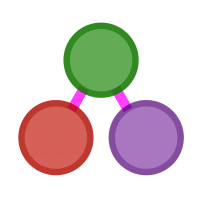
\includegraphics[width=11cm]{juliagraphs.png}}
% \caption{If necessary, the images can be extended both columns.}
%   \label{fig:sample_image}
% \end{figure*}

\section{Additional features}
\label{sec:additional_faci}
In addition to all the standard \LaTeX{} design elements, the \verb|juliacon|  class file includes the following features:
In general, once you have used the additional \verb|juliacon.cls| facilities
in your document, do not process it with a standard \LaTeX{} class
file.

\subsection{Titles, Author's Name, and Affiliation}
\label{subsub:title_auth}
The title of the article, author's name, and affiliation are used at the
beginning of the article (for the main title). These can be produced
using the following code:

\begin{verbatim}
\title{ This is an example of article title} }
\author{
   \large 1st Author \\[-3pt]
   \normalsize 1st author's affiliation  \\[-3pt]
    \normalsize 1st line of address \\[-3pt]
    \normalsize 2nd line of address \\[-3pt]
    \normalsize	1st author's email address \\[-3pt]
  \and
   \large 2nd Author \\[-3pt]
   \normalsize 2nd author's affiliation  \\[-3pt]
    \normalsize 1st line of address \\[-3pt]
    \normalsize 2nd line of address \\[-3pt]
    \normalsize	2nd author's email address \\[-3pt]
\and
   \large 3rd Author \\[-3pt]
   \normalsize 3rd author's affiliation  \\[-3pt]
    \normalsize 1st line of address \\[-3pt]
    \normalsize 2nd line of address \\[-3pt]
    \normalsize	3rd author's email address \\[-3pt]
}
\maketitle
\end{verbatim}

\subsection{Writing Julia code}

A special environment is already defined for Julia code,
built on top of \textit{listings} and \textit{jlcode}.

\begin{verbatim}
\begin{lstlisting}[
    language = Julia, 
    numbers=left, 
    label={lst:exmplg}, 
    caption={Example Code Block.}
]
using Plots

x = -3.0:0.01:3.0
y = rand(length(x))
plot(x, y)
\end{lstlisting}
\end{verbatim}
\begin{lstlisting}[
    language = Julia, 
    numbers=left, 
    label={lst:exmplg}, 
    caption={Example Code Block.}
]
using Plots

x = -3.0:0.01:3.0
y = rand(length(x))
plot(x, y)
\end{lstlisting}


\subsection{Abstracts, Key words, term etc...}
\label{subsub:abs_key_etc}

At the beginning of your article, the title should be generated
in the usual way using the \verb|\maketitle|  command. For genaral tem and keywords use
\verb|\terms|,
\verb|\keywords|  commands respectively. The abstract should be enclosed
within an abstract environment, All these environment
can be produced using the following code:
\begin{verbatim}
\terms{Experimentation, Human Factors}

\keywords{Face animation, image-based modelling...}

\begin{abstract}
In this paper, we propose a new method for the
systematic determination of the model's base of
time varying delay system. This method based on
the construction of the classification data related
to the considered system. The number, the orders,
the time delay and the parameters of the local
models are generated automatically without any
knowledge about the full operating range of the
process. The parametric identification of the local
models is realized by a new recursive algorithm for
on line identification of systems with unknown time
delay. The proposed algorithm allows simultaneous
estimation of time delay and parameters of
discrete-time systems. The effectiveness of
the new method has been illustrated through
simulation.
\end{abstract}

\end{verbatim}

\section{Some guidelines}
\label{sec:some_guide}
The following notes may help you achieve the best effects with the
\verb|juliacon|  class file.

\subsection{Sections}
\label{subsub:sections}
\LaTeXe{}  provides four levels of section headings and they are all
defined in the \verb|juliacon|  class file:
\begin{itemize}
\item \verb|\section|
\item \verb|\subsection|
\item \verb|\subsubsection|
\item \verb|\paragraph|
\end{itemize}
Section headings are automatically converted to allcaps style.
\subsection{Lists}
\label{sec:lists}
%
The \verb|juliacon|   class file provides unnumbered lists using the
\verb|unnumlist|  environment for example,

\begin{unnumlist}
\item First unnumbered item which has no label and is indented from the
left margin.
\item Second unnumbered item.
\item Third unnumbered item.
\end{unnumlist}
The unnumbered list which has no label and is indented from the
left margin. was produced by:
\begin{verbatim}
\begin{unnumlist}
\item First unnumbered item...
\item Second unnumbered item...
\item Third unnumbered item...
\end{unnumlist}
\end{verbatim}

The \verb|juliacon|  class file also provides hyphen list using the
\verb|itemize|  environment for example,
\begin{itemize}
\item First unnumbered bulleted item which has no label and is indented
from the left margin.
\item Second unnumbered bulleted item.
\item Third unnumbered bulleted item which has no label and is indented
from the left margin.
\end{itemize}
was produced by:
\begin{verbatim}
\begin{itemize}
\item First item...
\item Second item...
\item Third item...
\end{itemize}
\end{verbatim}

Numbered list is also provided in acmtog class file using the
enumerate environment for example,
\begin{enumerate}
\item The attenuated and diluted stellar radiation.
\item Scattered radiation, and
\item Reradiation from other grains.
\end{enumerate}

was produced by:
\begin{verbatim}
\begin{enumerate}
\item The attenuated...
\item Scattered radiation, and...
\item Reradiation from other grains...
\end{enumerate}
\end{verbatim}
\subsection{Illustrations (or figures)}
\label{subsub:sec_Illus}
The \verb|juliacon|  class file will cope with most of the positioning of
your illustrations and you should not normally use the optional positional
qualifiers on the \verb|figure|  environment that would override
these decisions.
\vskip 6pt

%
\begin{figure}[t]
\centerline{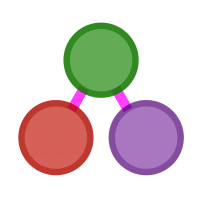
\includegraphics[width=4cm]{juliagraphs.png}}
\caption{This is example of the image in a column.}
	\label{fig:sample_figure}
\end{figure}

The figure \ref{fig:sample_figure} is taken from the JuliaGraphs
organization \footnote{https://github.com/JuliaGraphs}.

Figure captions should be \emph{below} the figure itself, therefore the
\verb|\caption|  command should appear after the figure or space left for
an illustration. For example, Figure 1 is produced using the following
commands:

\begin{verbatim}
\begin{figure}
\centerline{\includegraphics[width=20pc]{Graphics.eps}}
\caption{An example of the testing process for a
binary tree. The globa null hypothesis is tested
first at level $\alpha$ (a), and the level of
individual variables is reached last (d). Note
that individual hypotheses can be tested at
level $\alpha/4$ and not $\alpha/8$ as one might
expect at first.}
\label{sample-figure_2}
\end{figure}
\end{verbatim}
Figures can be resized using first and second argument of
\verb|\includegraphics|   command. First argument is used for modifying
figure height and the second argument is used for modifying
figure width respectively.
\vskip 6pt
Cross-referencing of figures, tables, and numbered, displayed
equations using the \verb|\label|  and \verb|\ref|   commands is encouraged.
For example, in referencing Figure 1 above, we used
\verb|Figure~\ref{sample-figure}|

 \subsection{Tables}
\label{subsub:sec_Tab}
The \verb|juliacon|   class file will cope with most of the positioning of
your tables and you should not normally use the optional positional qualifiers on the table environment which would override these
decisions. Table captions should be at the top.
\begin{verbatim}
\begin{table}
\tbl{Tuning Set and Testing Set}{
\begin{tabular}{|l|l|c|c|}\hline
Label & \multicolumn{1}{c|}{Description}
& Number of Users &
Number of Queries\\\hline
Train70 & Training Data &
\smash{\raise-7pt\hbox{70}} & 104\\
\cline{1-2}\cline{4-4}
Test70 & Testing Data I & & 105\\\hline
Test30 & Testing Data II & 30 & 119\\\hline
& Total & 100 & 328\\\hline
\end{tabular}}
\end{table}
\end{verbatim}

\begin{table}
\tbl{Tuning Set and Testing Set}{
\begin{tabular}{|l|l|c|c|}\hline
Label & \multicolumn{1}{c|}{Description}
& Number of Users &
Number of Queries\\\hline
Test 1 & Training Data &
\smash{\raise-7pt\hbox{70}} & 104\\
\cline{1-2}\cline{4-4}
Test 2 & Testing Data I & & 105\\\hline
Test 3 & Testing Data II & 30 & 119\\\hline
& Total & 100 & 328\\\hline
\end{tabular}}
\end{table}
\subsection{Landscaping Pages}
\label{subsub:landscaping_pages}
If a table is too wide to fit the standard measure, it may be turned,
with its caption, to 90 degrees. Landscape tables cannot be produced
directly using the \verb|juliacon|   class file because \TeX{} itself cannot
turn the page, and not all device drivers provide such a facility.
The following procedure can be used to produce such pages.
\vskip 6pt
Use the package \verb|rotating|   in your document and change the coding
from
\begin{verbatim}
\begin{table}...\end{table}
to
\begin{sidewaystable}...\end{sidewaystable}
and for figures
\begin{figure}...\end{figure}
to
\begin{sidewaysfigure}...\end{sidewaysfigure}
\end{verbatim}

environments in your document to turn your table on the appropriate
page of your document. For instance, the following code prints
a page with the running head, a message half way down and the
table number towards the bottom.
\begin{verbatim}
\begin{sidewaystable}
\tbl{Landscape table caption to go here.}{...}
\label{landtab}
\end{sidewaystable}
\end{verbatim}

\subsection{Double Column Figure and Tables}
\label{subsub:double_fig_tab}
For generating the output of figures and tables in double column
we can use the following coding:

\begin{enumerate}
\item For Figures:
\begin{verbatim}
\begin{figure*}...\end{figure*}
\end{verbatim}
\item For landscape figures:
\begin{verbatim}
\begin{sidewaysfigure*}...\end{sidewaysfigure*}
\end{verbatim}
\item For Tables:
\begin{verbatim}
\begin{table*}...\end{table*}
\end{verbatim}
\item For landscape tables:
\begin{verbatim}
\begin{sidewaystable*}...\end{sidewaystable*}
\end{verbatim}
\end{enumerate}

\subsection{Typesetting Mathematics}
\label{subsub:type_math}
The \verb|juliacon| class file will set displayed mathematics with center to
the column width, provided that you use the \LaTeXe{} standard of
open and closed square brackets as delimiters.
The equation
\[
\sum_{i=1}^p \lambda_i = (S)
\]

was typeset using the acmtog class file with the commands

\begin{verbatim}
\[
\sum_{i=1}^p \lambda_i = (S)
\]
\end{verbatim}

For display equations, cross-referencing is encouraged. For example,
\begin{verbatim}
\begin{equation}
(n-1)^{-1} \sum^n_{i=1} (X_i - \overline{X})^2.
\label{eq:samplevar}
\end{equation}
Equation~(\ref{eq:samplevar}) gives the formula for
sample variance.
\end{verbatim}
The following output is generated with the above coding:
\begin{equation}
(n-1)^{-1} \sum^n_{i=1} (X_i - \overline{X})^2.
\label{eq:samplevar}
\end{equation}
Equation~(\ref{eq:samplevar}) gives the formula for
sample variance.


\subsection{Enunciations}
\label{subsub:enunciation}
The \verb|juliacon|   class file generates the enunciations with the help of
the following commands:
\begin{verbatim}
\begin{theorem}...\end{theorem}
\begin{strategy}...\end{strategy}
\begin{property}...\end{property}
\begin{proposition}...\end{proposition}
\begin{lemma}...\end{lemma}
\begin{example}...\end{example}
\begin{proof}...\end{proof}
\begin{definition}...\end{definition}
\begin{algorithm}...\end{algorithm}
\begin{remark}...\end{remark}
\end{verbatim}
The above-mentioned coding can also include optional arguments
such as
\begin{verbatim}
\begin{theorem}[...]. Example for theorem:
\begin{theorem}[Generalized Poincare Conjecture]
Four score and seven ... created equal.
\end{theorem}
\end{verbatim}

\begin{theorem}[Generalized Poincare Conjecture]
Four score and seven years ago our fathers brought forth,
upon this continent, a new nation, conceived in Liberty,
 and dedicated to the proposition that all men are
created equal.
\end{theorem}


\subsection{Extract}
\label{subsub:extract}
Extract environment should be coded within
\begin{verbatim}
\begin{extract}..\end{extract}
\end{verbatim}

\subsection{Balancing column at last page}
\label{subsub:Balance}
For balancing the both column length at last page use :
\begin{verbatim}
\vadjust{\vfill\pagebreak}
\end{verbatim}

%\vadjust{\vfill\pagebreak}

at appropriate place in your \TeX{} file or in bibliography file.

\section{Handling references}
\label{subsub:references}
References are most easily (and correctly) generated using the
BIBTEX, which is easily invoked via
\begin{verbatim}
\bibliographystyle{juliacon}
\bibliography{ref}
\end{verbatim}
When submitting the document source (.tex) file to external
parties, the ref.bib file should be sent with it.
\cite{bezanson2017julia}

% **************GENERATED FILE, DO NOT EDIT**************

\bibliographystyle{juliacon}
\bibliography{ref.bib}


\end{document}

% Inspired by the International Journal of Computer Applications template
